\section{Quantifying Baryon Redistribution}
\label{sec:feedbackmetrics}

Feedback is a complex process that impacts a wide range of
baryonic observables, from the galaxy stellar mass function, to galaxy sizes,
to the density profiles of galaxies \citep[e.g.][]{BenitezLlambay2018}. It is
interesting, therefore, to develop tools to study the global effects of
feedback directly, as a complement to the many indirect constraints
obtainable from comparing to astrophysical observables. Here we describe the
tools we will use to examine the redistribution of baryons via feedback.

The kinetic feedback scheme used in \simba{} for both star formation and AGN
feedback makes it straightforward to identify the gas elements that have been
directly impacted by feedback. However, these gas elements will then go on to
entrain and deposit energy into other gas elements as they travel. This makes
it challenging to fully capture the impact of feedback solely from particle
tagging. Another option to assess feedback is to run simulations with
specific feedback modules turned on and off. However, this is inconsistent
with the tuning procedure that virtually every simulation suite performs in
order to constrain the many parameters in the sub-grid model. For instance,
modern models are typically calibrated to the $z=0$ Stellar Mass Function
(SMF), which will of course change should some feedback mechanism be missing
(and hence should be re-calibrated). It is thus important to realize that, if
without some feedback module a simulation fails to match data, this does not
definitively prove that the feedback module is necessary to produce realistic
galaxies, since it could potentially be that the simulation could be
recalibrated to match data in some other way. In our case, we run the \nojet{}
and non-radiative variants in order to explore how baryon redistribution is
sensitive to these feedback modules, but we do not attempt to recalibrate
these to data, and merely use them in order to investigate the impact of this
input physics within the context of the \simba{} model.

% These are all together to ensure they end up on the correct pages, sorry.

\subsection{The Spread Metric}

\begin{figure}
    \centering
    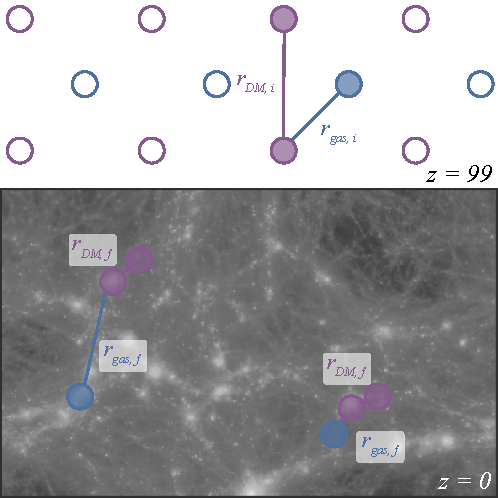
\includegraphics[width=\columnwidth]{figures/kspafig_small.pdf}
    \vspace{-0.5cm}
    \caption{The matching procedure between initial and final conditions
    illustrated. The top panel shows the $z=99$ initial conditions, where
    every particle finds its nearest dark matter neighbour. The bottom
    panel shows the distances between those particles at $z=0$. For the
    fiducial result, each particle actually finds the three nearest 
    neighbours in the initial conditions and takes the median at $z=0$
    of these distances (see text for explanation) but this is omitted
    in this simple picture for brevity.}
    \vspace{-0.5cm}
    \label{fig:kspafigsmall}
\end{figure}

Our approach to quantifying the large-scale impact of feedback is to develop
a simple and robust metric that directly captures the displacement of the gas
owing to feedback. This `spread' metric, illustrated in Figure
\ref{fig:kspafigsmall}, works as follows:

\begin{enumerate} 
	\item For every particle $i$ in the initial conditions, find the nearest
          $n$ dark matter neighbours $j$ (with $n=3$ for the fiducial result).
	\item In the final conditions, match all remaining baryonic particles
	      with their initial conditions progenitor (in this case, stars are
	      matched with their gas progenitor).
	\item In the final conditions, find the distance $r_{ij}$, i.e. the
	      distance between the particle and its original neighbours. The spread metric for
	      this particle is then given as the \emph{median} of these $n$
	      distances.
\end{enumerate}

\begin{figure}
    \centering
    \includegraphics{report/figures/s50j7k/dark_matter_distance_figure_s50j7k.pdf}
    \vspace{-0.5cm}
    \caption{Shows the distribution of final-state distances from the spread
             metric for dark matter in the full \simba{} model run. This distribution
             is relatively unchanged by the choice of sub-grid
             model, and the effects of the back-reaction of baryonic physics on dark
             matter is out of the scope of this work. The distribution is split
             between particles that lie within halos and those that lie outside, with
             this being an approcimately even split at $z=0$. Lines are over-plotted
             to show the maximal distance between any two dark matter particles at $z=0$,
             approximately $0.5\hmpc{}$, and twice the maximal virial radius of any halo 
             in the box, which is approximately $1.3\hmpc{}$. The inset figure
             shows the inner $0.5\hmpc{}$ of the distribution, and has a line over-plotted
             for the mean inter-particle separation in the initial conditions (MIPS)
             of approximately $0.1\hmpc$. The fainter lines show how the short-distance
             distribution changes when taking the average over a number of initial nearest
             neighbours; dashed gives the metric with no median (i.e. only one nearest
             neighbour), and the dotted line shows the case for a median over 9 neighbours.
            }
    \vspace{-0.5cm}
    \label{fig:dmonlyspread}
\end{figure}

The `spread' metric is presented first for dark matter in Figure \ref{fig:dmonlyspread}.
The simplest metric here clearly is simply to use the nearest neighbour in the
initial conditions, rather than the median over $n$ initial neighbours. The
choice of $n=3$ was made primarily to ensure that the dark matter results were
robust when comparing matter inside and outside of halos. For a given
dark matter particle pairing, a large distance between two neighbours
would be `double counted' for the case where one neighbour makes it into
a halo and one remains outside, contributing the large distances to both
bins. Choosing $n=3$ enables the median result to actually represent the
distance to a full particle, and removes the problem of the double counting
for the nearest neighbour. The overall distributions of distances, however,
were not changed much by this choice. It does increase the contrast in the
dark matter images in Figure \ref{fig:bigdistanceimage}, with more substructure
being picked up in the low-distance particles, and more diffuse structure in the
large-distance particles, with an increasing number of neighbours.

\begin{figure*}
    \centering
    \vspace{1cm}
    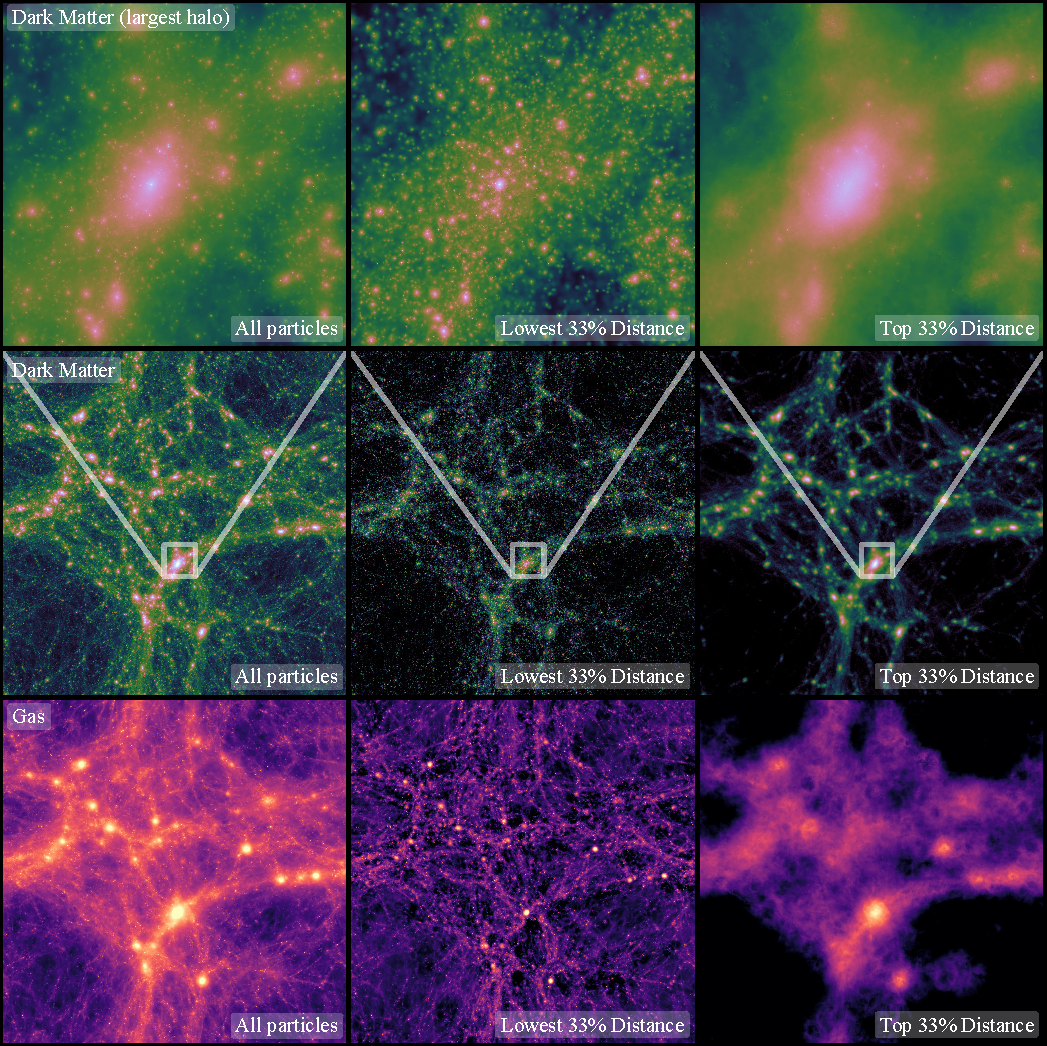
\includegraphics[width=\textwidth]{report/figures/distance_figures_3.pdf}
    \caption{The three rows show the following selections of particles (from top to bottom):
        the dark matter present in the largest halo, and surrounding it (this is a $4.5\hmpc{}$
        cube centered around the halo centre, which has a virial radius of approximately $1.3\hmpc{}$);
        all dark matter particles in the box; and all gas particles present in the box. All images
        are shown in the final state of the simulation at redshift $z=0$. Each column then shows
        (from left to right): all particles that are in the volume; the particles that have spread
        the least, selecting the first 33\% from the histogram figures; and the particles that have
        spread the 33\% most. For the dark matter, these cuts correspond to particles that have travelled
        less than $0.1\hmpc{}$, and greater than $0.25\hmpc{}$ respectively. For the gas, these numbers
        increase to $0.45\hmpc{}$ and $1.25\hmpc{}$ respectively due to the larger spread that these
        praticles expereice. Each image has smoothing lengths generated to encompass $32$ nearest
        neighbours, as is used in the \simba{} simulations, and smoothing lengths are kept consistent
        across columns; i.e. they are not re-smoothed. All images in a given row also use the exact
        same (logarithmic) normalisation and colour map to enable comparisons. Note how even with this
        extremely conservative cut there is a significant difference between the images, with sub-structure
        picked out by the low-distance cut and large-scale structure for the large-distance cut.}
    \vspace{1cm}
    \label{fig:bigdistanceimage}
\end{figure*}


Figure \ref{fig:feedbackpic} visualizes how this metric looks in our \simba{}
simulation. This metric shows the extreme distances that feedback processes
can cause baryons to be ejected to. Note that the colour bar for distance
shows separations of over $10\hmpc{}$. The background gas density map shows
the positions of halos in the simulation; note that the majority of particles
that are ejected to large distances (relative to their dark matter) end up
far outside any of the large halos. The metric also shows that the central
galaxies of the halos are predominantly made up of tightly bound baryons and
dark matter (i.e. the baryons in these halos have not moved very far relative
to their closest dark matter neighbour in the initial conditions). This again
re-enforces the view that central galaxies initially form out of the gas made
up of their halo, but feedback processes cause outflows of gaseous material
that both pollutes the CGM and IGM surrounding that halo and may find its way
into other halos.

\subsection{Baryon Spreading in \simba{}}

\begin{figure}
    \centering
    \includegraphics{report/figures/s50j7k/distance_plot_split_by_component.pdf}
    \vspace{-0.5cm}
    \caption{The distance metric histogram, now including gaseous matter. Note how,
    compared to the dark matter, the distributions for gas inside halos and outside
    halos are significantly different, with gas that originated in lagrangian regions
    being preferentially moved to larger distances than gas on average. Note that only
    10\% of the gas in the entire simulation is in halos at $z=0$. Gas can be blown
    out to $12\hmpc{}$, approximately 10 times the virial radius of the largest halo
    in the box.
    \blue{TODO: Change the normalisation here to be the same as above}.}
    \vspace{-0.5cm}
    \label{fig:distbaryon}
\end{figure}

Now considering the baryons in the simulation in Figure \ref{fig:distbaryon}.

\begin{figure*}
    \centering
    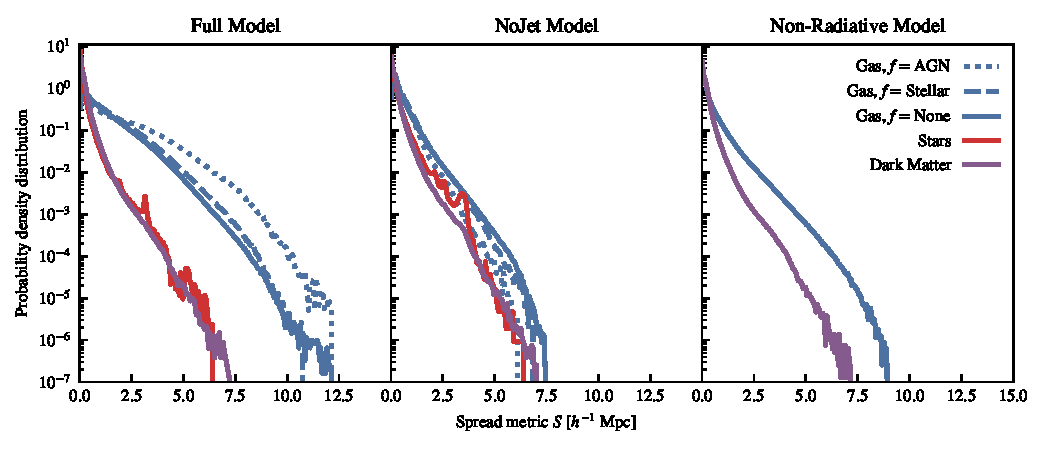
\includegraphics[width=\textwidth]{figures/neighbour_analysis_feedback_histogram_combined.pdf}
    \vspace{-0.7cm}
    \caption{
        The (normalised) distribution of distances for all particles $i$ to
        the nearest neighbour $j$ in the initial conditions, split by particle
        type. This is shown for the $z=0$ particle distribution in the
        reference model (left), \nojet{} model (center), and a non-radiative
        run (right). Splitting the particles by those that have been
        involved in feedback events in this figure shows that the further
        out a particle has been blown the more likely it is to have been
        directly involved in a feedback event for the reference model. Also note
        the vertical $0.5-1$ dex offset for gas compared to dark matter even in
        the \nojet{} run. \blue{TODO: Change the normalisation here}.
    }\label{fig:feedbackdistance}
\end{figure*}

In Figure \ref{fig:feedbackdistance} (left panel) the distribution of
distances in the reference model is shown. Note how similar the stellar
distribution is to the dark matter distribution even though strong feedback
is included. From this we conclude that star particles are mainly formed out
of tightly bound gas (this is ensured almost by construction due to the
density criterion in the sub-grid model) that is unable to separate
dynamically from the dark matter. Also, the peak of star formation is far
before redshift $z=0$ and so it is unsurprising that the stellar dynamics
have relaxed back to something similar to the dark matter despite starting
out life as gas. The maximal distance of around $6\hmpc{}$ is expected, as it
is about three times the virial radius of the largest halo in the simulation;
a pair of initially neighbouring particles can end up on opposite sides of a
given halo. Matter that remains in a gaseous state, on the other hand, can be
blown out to very large distances (over $12 \hmpc{}$).

Comparing to the \nojet{} run in Figure \ref{fig:feedbackdistance}, it is clear
that the jets have a significant impact on the distances to which particles
are spread. These two plots show directly the issue of entrainment that was
raised earlier; the tail is expanded to include lots of gas that was never
tagged as having been included in any feedback event.

The significant difference in the dynamics between the \nojet{} run and the
reference model is surprising. Less than $0.4\%$ of gas particles in the simulation
have ever interacted directly with the AGN jets; this has been enough
to completely separate the majority of the gas from the dark matter dynamically.
Such a high degree of separation points to huge amounts of gas being entrained
by these powerful jets. It is not simply the case that higher mass ($M_H >
10^{11} \msolar{}$) halos are quenched internally reducing their star formation
rate; the energetics and dynamics of the CGM and IGM are significantly altered
leading to a much more complex interaction between the turn-off of the
galaxy stellar mass function (GSMF) and the power of the AGN jets.

The final contrast to highlight is the difference between the \nojet{} and
non-radiative model. The non-radiative model shows increased distance between
gas particles and their associated dark matter neighbour compared to the
\nojet{} run; this is likely due to the lack of cooling preventing particles
that lie in small halos from remaining as tightly bound.

\begin{figure}
    \centering
    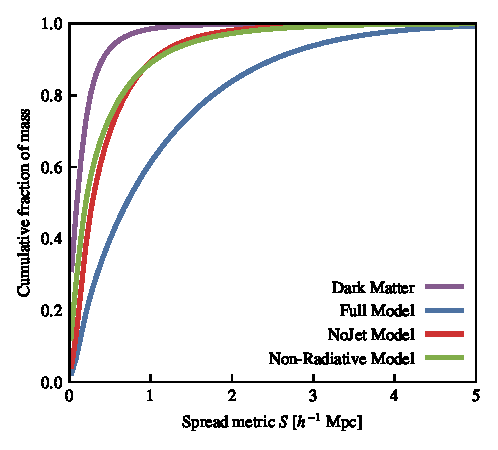
\includegraphics{figures/cumulative_histogram_comparison.pdf}
    \vspace{-0.7cm}
    \caption{Cumulative version of Fig. \ref{fig:feedbackdistance} that
    shows the gas distribution for the three models alongside the dark
    matter from the full model.}
    \label{fig:cumulativehistogram}
\end{figure}

In Fig. \ref{fig:cumulativehistogram} we show the cumulative version of Fig. 
\ref{fig:feedbackdistance} to show that it is not a negligible amount of mass
that is entrained by the full model out ot large distances. Only 90\% of gaseous
mass is constrained within $3\hmpc{}$.

These results show that gaseous and stellar matter can be transferred out
to significantly further (by $z=0$) than is assumed by typical zoom-in simulation
suites. For example, the Latte \citep{Wetzel2016} suite uses an exclusion region
for high resolution particles of around $1.5 \hmpc{}$. Whilst they do not find
contamination (possibly due to refinement criteria) of low-resolution particles
into the high-resolution region, the above metrics suggest that perhaps this is
a more numerical, rather than physical, effect; low resolution particles are
not present due to a lack of sub-grid physics in the unrefined region.
